\documentclass[11pt]{article}
\usepackage{enumerate}
\usepackage{amsfonts}
\usepackage{amsmath}
\usepackage{mathabx}

\usepackage{graphicx}


% Allows me to align the top of images with enumerate
\usepackage[export]{adjustbox}

% makes quotation marks show up correctly
\usepackage [english]{babel}
\usepackage [autostyle, english = american]{csquotes}
\MakeOuterQuote{"}

\begin{document}

\let\iff\leftrightarrow

\title{Com Sci 330 Assignment 12}
\author{Adam Hammes, hammesa@iastaste.edu}
\maketitle


\section*{Problem 1}
\begin{enumerate}[(a)]
	\item	
	Since the set is between $1,000$ and $9,999$ inclusive, the size of the set is $9,999\ -1,000 +1 = 9,000$. To find the number of integers in that set that contain at least one 0 and one 1, we will find the number of integers in that range that don't have those digits and subtract from 9,000.
	
	In the case of the numbers with no 1, there are 8 possibilities for the first digit ($n \ge 1000$ implies first digit is $\neq 0$), and 9 possibilities for the other three digits, for a total of $8 \times 9^5 = 5,832$ integers. For the numbers with no 0, there are nine possibilities for each of the four digits for a total of $9^4 = 6,561$ integers. Adding these numbers yields 12,393 integers.
	
	The previous two sets double-count a lot of numbers, such as 9,999. To account for this, we need to subtract from the previous number the intersection of two sets; that is, numbers that don't contain 0 and don't contain 1. Each digit of these numbers has 8 possible values, for a total $8^4 = 4,096$ double-counted numbers. Therefore the number of integers $1,000 \le n \le 9,999$ is $9,000 -(12,393 - 4,096) = 703$.

	\item
	Let $A$ contain all integers $1,000 \le n \le 9,999$ with at least one 0, $B$ at least one 1, and $C$ at least one 2. The formula given in the problem allows us to calculate the union of these sets with the following formula:
	\begin{equation}
	|A \cup B \cup C| = |A| + |B| + |C| - |A \cap B| - |A \cap C| - |B \cap C| + |A \cap B \cap C|
	\end{equation}
	To calculate the size of these sets, I will subtract the number of integers that *aren't* in the set and subtract from the size of the range, 9,000, similar to what I did in part (a).
	
	$|A|$ - calculated in (a); $9,000 - 6,561 = 2,439$.
	
	$|B|$ - calculated in (a); $9,000 -5,832 = 3,168$.
	
	$|C|$ - $|\bar{C}|$ has 9 possibilities has nine possibilities for each of the digits except the first, which has eight (since the first digit can't be zero); $9,000 - 8\times 9^3 = 3,158$.
	
	$|A \cap B|$ - calculated in (a); 703.
	
	$|A \cap C|$ - since $|C|= |B|$, $|A \cap C| = |A \cap B| = 703$.
	
	$|B \cap C|$ - $|\bar{B} \cap \bar{C}|$ has $10-2 =8 $ possibilities for each of the digits except of the first, which has seven (since the first digit can't be zero); $9,000 - 7\times 8^3 = 5416$; this is the number of double-counted possibilities, which we subtract from $|B| + |C|$. $3168\times 2 - 5416 = 920$.
	
	$|A \cap B \cap C$ - again, find all the numbers not in this set, numbers with no 0, 1, or 2. Seven possibilities for each digit, so the size is $7^4 = 2401$.
	
	Plugging the numbers back into the formula gives $2,439 + 3,168 + 3,168 - 703 - 703 - 920 + 2,401 = 8850$.
	
\end{enumerate}


\section*{Problem 2}

$G$ is a simple, undirected graph, so each edge consists of a pair of distinct vertices. Therefore each edge increases the degrees of two vertices by one. This implies that the sum of the degrees of the vertices of a graph is twice $|E|$. Since the sum of degrees in $G$ is $5+5+3+3+2+2 = 20$, there are $20 \div 2 = 10$ edges in the graph.

\section*{Problem 3}

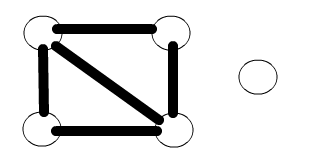
\includegraphics[scale=.5]{images/p3}\\
There are 5 vertices and 5 edges, but the vertex on the right is not connected. Therefore for a graph $G = (V,\ E)$, $|V| = |E|$ does not imply that $G$ is connected.

\section*{Problem 4}
I'll prove the biconditional both ways separately.\\\\
Tree $\implies$ connected and removing one edge will disconnect the graph.\\

There are two requirements for a graph to be a tree; it has to be connected and acyclic. Let $G$ be a graph. If $G$ is a tree, it is obviously connected. Assume for sake of contradiction that removing an edge will not disconnect the graph, and let this edge be $(u,\ v)$ where $u,\ v$ are any two vertices in $G$. Since the graph obtained from removing an edge is connected, there exists a path between $u$ and $v$; if we consider the edge we just removed, there are actually two paths from $u$ to $v$ in $G$, a contradiction because $G$ is acyclic. Therefore if $G$ is a tree then removing one edge will disconnect the graph.\\\\
Connected and removing one edge disconnects the graph $\implies$ $G$ is a tree.\\

Let $G= (V,\ E)$ be a connected graph, and removing any edge $e \in E$ disconnects the graph. We have to prove two conditions to determine that $G$ is a tree - $G$ is connected and $G$ is acyclic. Since $G$ is connected, we have already satisfied the first condition. Since $\forall e \in E$, removing $e$ disconnects two vertices $u, v \in V$, there exists only one path between $u,\ v$. This implies that between any two vertices there exists only one path, so $G$ is acyclic. QED.


\section*{Problem 5}

\begin{enumerate}[(a)]
	\item
		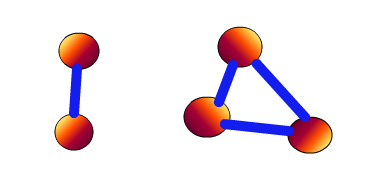
\includegraphics[scale=.5, valign = t]{images/p5}\\
	The left two vertices both have one edge, and every other vertex has two edges; therefore the graph is two-ended. However, it is not possible to list the vertices as a sequence with edges between consecutive vertices only because the vertices on the right form a cycle. So, by definition, the graph is not a line graph.
	
	\item
	The proof assumes that a two-ended graph with $n+1$ edges can be formed from a two-ended graph of $n$ edges. However, the graph depicted in part (a) has four edges but cannot be formed by adding an edge to a graph with three edges. Removing an edge from the left side creates a graph with two vertices with an edge count of 0, which is not two-ended; removing an edge from the right side breaks the cycle, leaving the graph with four vertices with one edge, which is also not two-ended. \\\\
	Since the graph cannot be formed by induction on the number of edges, the proof does not consider all possible two-ended graphs and is therefore erroneous. QED. 
	
\section*{Problem 6}

Not attempted.

\end{enumerate}

\end{document}